\chapter{Experiments}

The purpose of experiments is to observe common patterns, that allow a better understanding of the system, which may be used for optimization, customization and improvement needs. In this chapter will be studied the benefits, which may be achieved be applying parallelization to any of the used algorithms.

\section{Testing environment}

In order to run experiments objectively and make fair conclusions, it is important to set the testing environment, which is going to be the same for every test run.

\subsection{Settings}

The experiments will be performed on one of the implemented examples of library usage. This is the solution for the Quadratic Assignment Problem. It is one of the fundamental combinatorial optimization problems in the branch of optimization or operations research in mathematics, from the category of the facilities location problems. For this purposes could have been used any problem, as in order to make conclusions, the results will be compared with each other.

Here is a list of the parameters mutual to every test:
\begin{itemize}

\item Optimization problem

The experiments will be performed on one of the implemented examples of library usage -  Quadratic Assignment Problem. It is one of the fundamental combinatorial optimization problems in the branch of optimization or operations research in mathematics, from the category of the facilities location problems. For this purposes could have been used any problem, as in order to make conclusions, the results will be compared with each other.


\item Genetic operators

For the evolution flow, the set operators stay unchanged. It contains tournament selection strategy with the size of 20, one point crossover and simple chromosome swap mutation. These parameters have been left immutable in order to minimize parameter noise during experiments.

\end{itemize}

Other algorithm parameters like the number of iterations, size of the population and complexity of fitness function will be regularized in order to examine the correlation.

\subsection{Hardware}

The experiments were performed using two machines with a different configuration, motivated by the different results, which may be observed depending on the used machine.

\begin{table}[h]
\centering\caption{Hardware characteristics \label{tab:exp-hardware}}
\begin{tabular}{|l|c|c|c|}
\hline
\textbf{Label} & \textbf{Operating system} & \textbf{Total RAM} & \textbf{vCPU cores} \\
\hline
Machine \#1 & Windows 10 & 16 GB & 8 \\
\hline
Machine \#2 & Ubuntu 18.04 & 8 GB & 4 \\
\hline
\end{tabular}
\end{table}

\section{Sequential behavior}

In order to be able to make some conclusions having the data from experiment runs, it is important to know how the system behaves in sequential runs. This configuration may also be considered as one with parallelism level 1.

Run parameters:
\begin{table}[h]
\centering\caption{Hardware characteristics \label{tab:exp-hardware}}
\begin{tabular}{|l|c|c|c|}
\hline
\textbf{Parameter} & \textbf{Value}  \\
\hline
Number of iterations & 10 \\
\hline
Size of population & 5000 \\
\hline
Fitness function duration & ~5 ms \\
\hline
\end{tabular}
\end{table}

After the run with a sequential implementation of GA here is a plot of processor resources usage over time \ref{img:cpu-run-1}. It is clear that only one virtual CPU core is working on its full speed at a time, but there is no virtual CPU core, which runs all the evolution, as after some time it is changed to another core. In the meanwhile, there bumps on other cores every some time. This is garbage collector sessions, as by default JVM runs GC on the free cores in order to minimize actual working time.

\begin{figure}[h]
\centering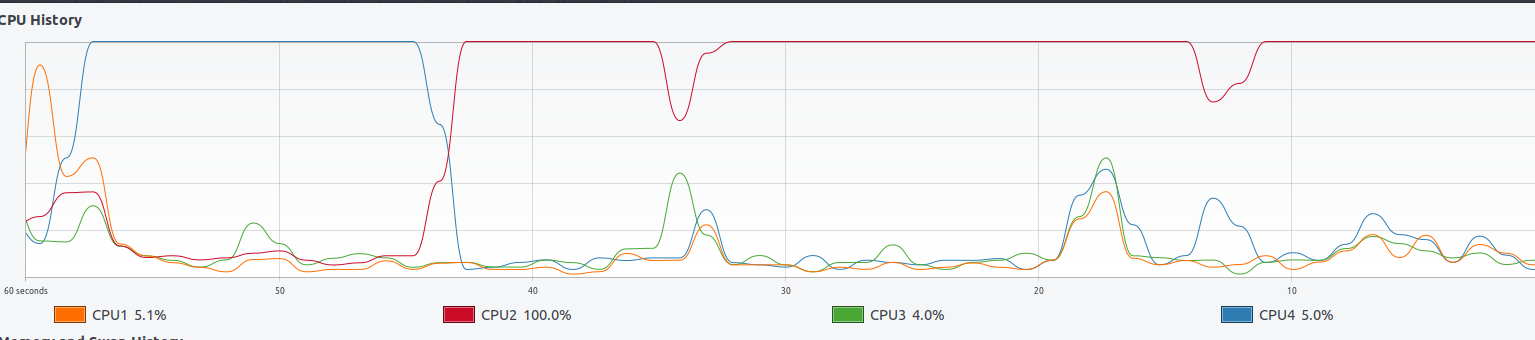
\includegraphics[width=1\textwidth]{img/exp/1/cpu-500}
\caption{CPU load during test run \#1}  \label{img:cpu-run-1}
\end{figure}

To test whether conjecture about GC runs is actually true for the next run the size of a population was increased to 50000 and fitness function time reduced to 0.5 ms. This should increase the number of objects allocated during a given time segment, resulting in more frequent garbage collector sessions. Here are the observations over CPU status during the run \#2 \ref{img:cpu-run-2}. This plot confirms the previous assumption - number of load rises is much bigger, as a lot more object are allocated and deallocated. Nevertheless, CPU usage in example \#2 in some aspects is similar to the CPU usage during run \#1: there is only one virtual CPU working for 100\% at a time and the rest of virtual cores are working on additional job, such as garbage collection or scheduling.

\begin{figure}[h]
\centering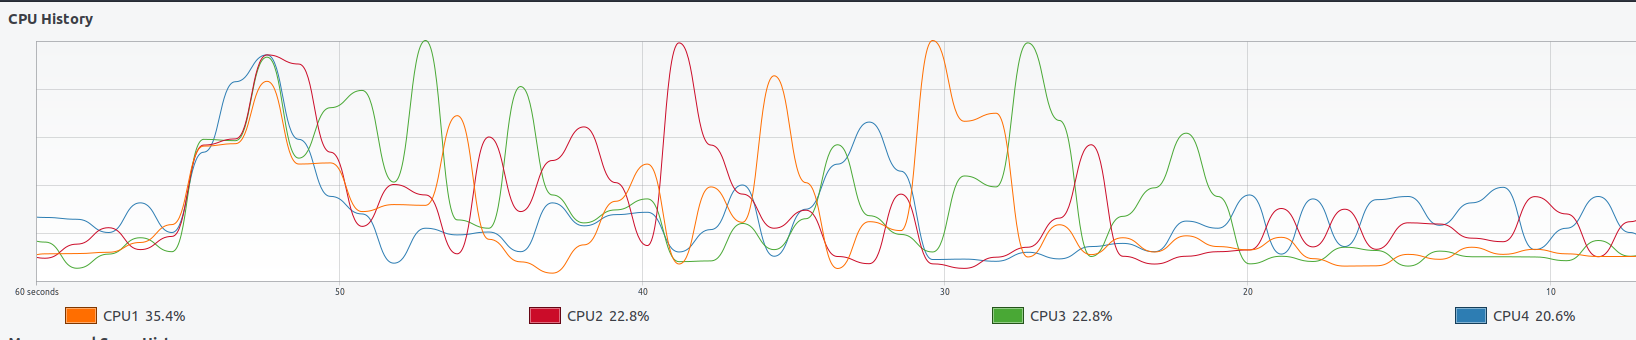
\includegraphics[width=1\textwidth]{img/exp/1/cpu-5000}
\caption{CPU load during test run \#2}  \label{img:cpu-run-2}
\end{figure}

The important conclusion from these runs is that even during sequential computations JVM still uses other available cores to optimize working time. For this reason, when using more than one CPU core for the purpose of an algorithm, JVM may find no free cores and will schedule garbage collection together with other computations, which will naturally result in a downturn of performance. \textbf{This is one of the reasons, why the speed-up from parallelization is not ideally linear to the number of added cores.}


\section{Measuring parallelization impact}

In this section will be measured performance increase in different thread pool configuration.
Performance of each configuration will be measured and compared to the performance of sequential run without thread pool limitation. The goal of the experiment is to find what kind of configuration provides the best performance characteristics of the algorithm.

\subsection{Performance increase}

By applying a thread pool, depending on its type, an application is restricted to use no more or exact number of threads to its purposes. This also includes garbage collection, so the statement that sequential run is equal to parallel with limited pool to one thread is not true, as in the former case garbage collection may be scheduled on the other thread by JVM, wherein the letter - one thread is responsible for all actions. This is why parallelization with a small number of threads gives a very small speed-up.

The measurements can be found in tables \ref{tab:comp-ubuntu} and \ref{tab:comp-windows} in comparison to sequential run values placed in \ref{tab:win-ub-perf}.

\begin{table}[h]
\centering\caption{Performance of sequential configuration of genetic algorithm \label{tab:win-ub-perf}}
\begin{tabular}{|c|c|c|c|}
\hline
\textbf{Machine} & \textbf{Taken time} & \textbf{Population size} \\
\hline
Machine \#1 & 1725 ms & 10000 \\
\hline
Machine \#2 & 1779 ms & 10000 \\
\hline
\end{tabular}
\end{table}

\begin{table}[H]
\centering\caption{Performance speedup depending on available threads comparing with sequential run on machine \#1 \label{tab:comp-windows}}
\begin{tabular}{|c|c|c|c|}
\hline
\textbf{Number of threads in the pool} & \textbf{Taken time} & \textbf{Performance increase} & Available vCPU cores \\
\hline
2 & 1276 ms & 35.2\% & 8 \\
\hline
4 & 509 ms & 238\% & 8  \\
\hline
8 & 345 ms & 400\% & 8 \\
\hline
16 & 328 ms & 426\% & 8 \\
\hline
32 & 296 ms & 482.7\% & 8 \\
\hline
64 & 300 ms & 475\% & 8 \\
\hline
100 & 305 ms & 465.6\% & 8 \\
\hline
\end{tabular}
\end{table}

\begin{table}[h]
\centering\caption{Performance speedup depending on available threads comparing with sequential run on machine \#2 \label{tab:comp-ubuntu}}
\begin{tabular}{|c|c|c|c|}
\hline
\textbf{Number of threads in the pool} & \textbf{Taken time} & \textbf{Performance increase} & Available vCPU cores \\
\hline
 2 & 1247 ms & 42.6\% & 4 \\
\hline
 4 & 640 ms & 177\% & 4 \\
\hline
 8 & 564 ms & 215\% & 4 \\
\hline
 16 & 576 ms & 208\% & 4 \\
\hline
 32 & 592 ms & 200.5\% & 4 \\
\hline
\end{tabular}
\end{table}

Using graph visualizations \ref{img:ub-perf}, \ref{img:win-perf} it is shown, that slope of performance increase is independent from machine or operating system. 

\begin{figure}[H]
\centering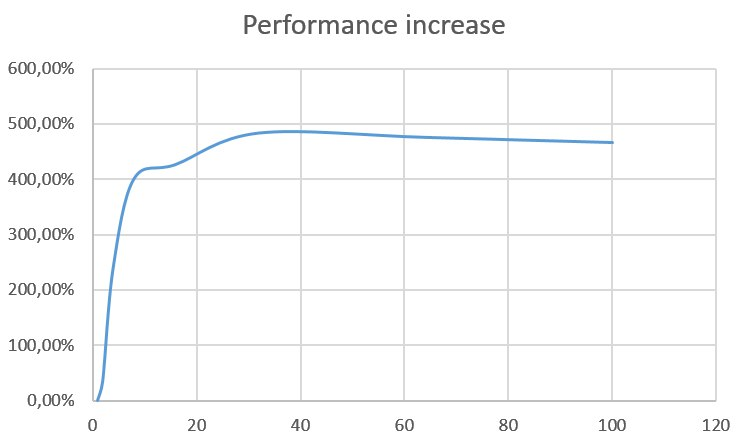
\includegraphics[width=.8\textwidth]{img/exp/2/windows-performance-increase}
\caption{Visualization of performance increase per available threads on machine \#1}  \label{img:win-perf}
\end{figure}

\begin{figure}[h]
\centering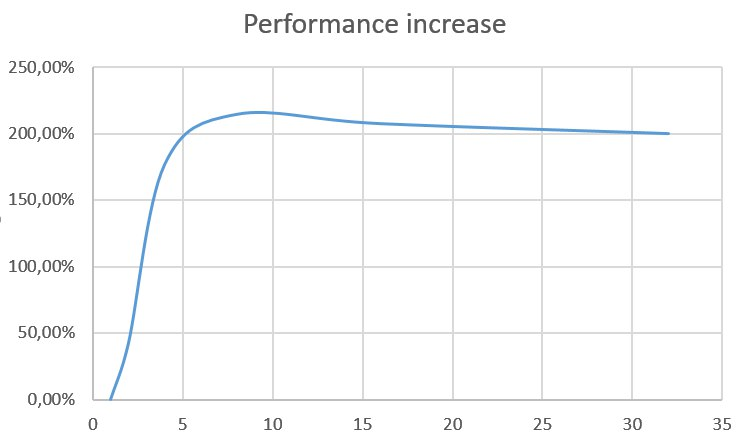
\includegraphics[width=.8\textwidth]{img/exp/2/ubuntu-performance-increase}
\caption{Visualization of performance increase per available threads on machine \#2}  \label{img:ub-perf}
\end{figure}

From observations it also appears, that \textbf{optimal point of performance gain is approximate to \( 2 * n\) threads available in case of the fixed thread pool, where \(n\) is number of virtual CPU cores available on the machine.}

\subsection{CPU Load}

While testing how different thread pools applied to an application change its overall performance, machine CPU load was measured in order to better understand the nature of speed-up. There are screenshots from the resource monitoring tool, taken while running the application with different configurations \ref{img:cpu-thread-2}, \ref{img:cpu-thread-4}, \ref{img:cpu-thread-8}, \ref{img:cpu-thread-16}, \ref{img:cpu-thread-32} (all runs were performed on machine \#2 with 4 virtual CPU cores).

\begin{figure}[h]
\centering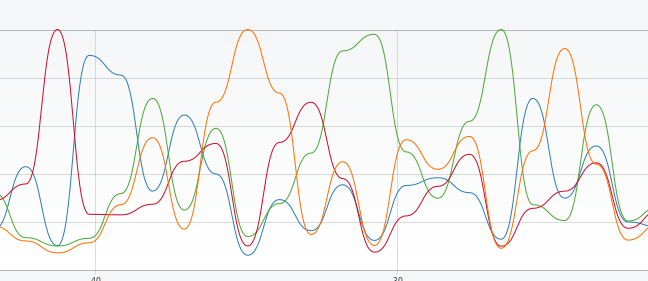
\includegraphics[width=0.95\textwidth]{img/exp/2/limit-threadpool-2}
\caption{The CPU load while processing GA evolution limited by a thread pool with fixed size 2 }  \label{img:cpu-thread-2}
\end{figure}

\begin{figure}[H]
\centering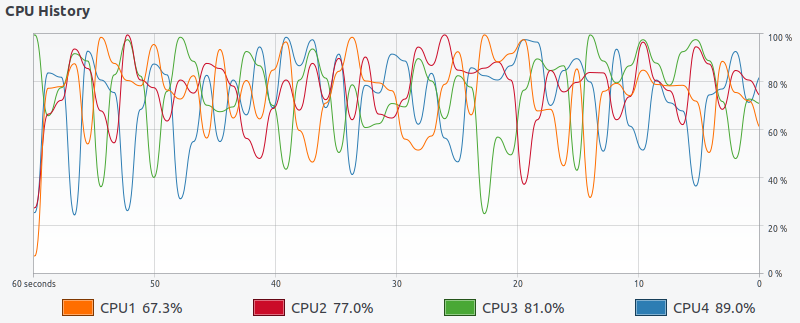
\includegraphics[width=0.95\textwidth]{img/exp/2/limit-threadpool-4}
\caption{The CPU load while processing GA evolution limited by a thread pool with fixed size 4 }  \label{img:cpu-thread-4}
\end{figure}

\begin{figure}[H]
\centering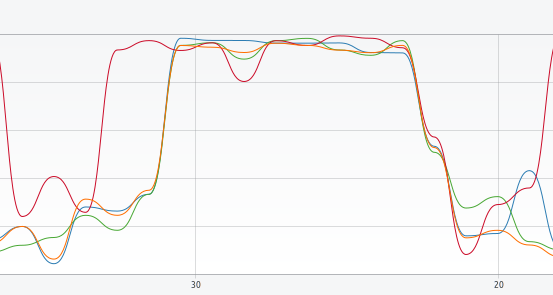
\includegraphics[width=0.95\textwidth]{img/exp/2/limit-threadpool-8}
\caption{The CPU load while processing GA evolution limited by a thread pool with fixed size 8 }  \label{img:cpu-thread-8}
\end{figure}

\begin{figure}[H]
\centering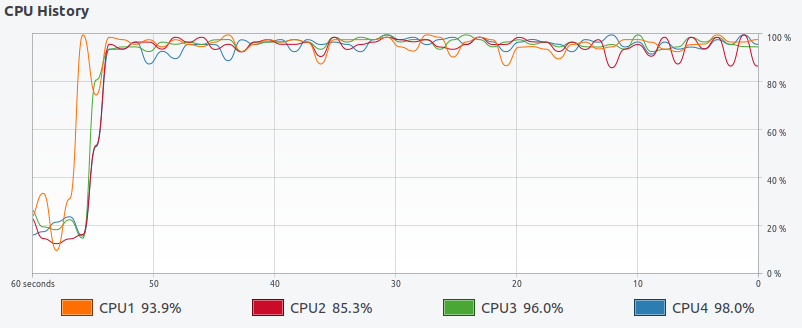
\includegraphics[width=0.95\textwidth]{img/exp/2/limit-threadpool-16}
\caption{The CPU load while processing GA evolution limited by a thread pool with fixed size 16 }  \label{img:cpu-thread-16}
\end{figure}

\begin{figure}[H]
\centering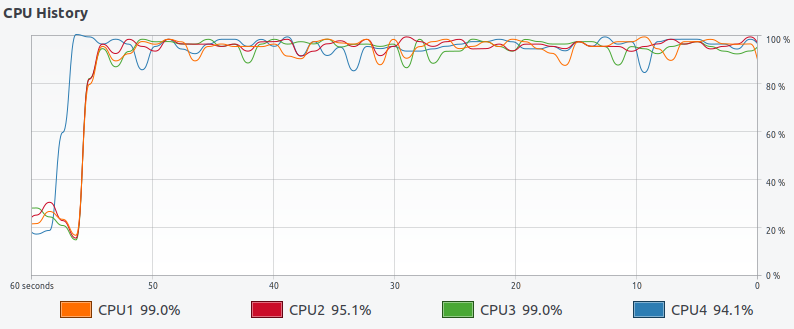
\includegraphics[width=0.95\textwidth]{img/exp/2/limit-threadpool-32}
\caption{The CPU load while processing GA evolution limited by a thread pool with fixed size 32 }  \label{img:cpu-thread-32}
\end{figure}

These plots correspond to the virtual CPU cores workloads during the algorithm run. In order to achieve the highest performance, the maximum amount of work should be done in a time segment, so the CPU load should be the highest. When applying a  thread pool with 2 available threads, having 4 virtual CPU cores, task scheduler is jumping from one core to another, keeping average CPU load near 60\%. This confirms low-performance increase, comparing to bigger thread pools. Later with each next thread pool configuration applied the average CPU load increases with the number of available threads, reaching its peak with 16-thread pool on 95\% (some of the resources are reserved for the operating system, preventing running processes - JVM in this case - from corrupting machine state). When running the application on 32 threads, which is 8 times more than available virtual CPU cores, average CPU load is nearly the same, with more resources assigned to keep the thread scheduling, which together corresponds to the smaller performance gain, compared to a 16-thread pool. On this level parallelization job scheduling and switching between different tasks are taking more resources, which could have been used for ``business'' computations. \textbf{Basing on these observations, running the application with minimum I/O manipulations, it is optimal to keep the number of threads per virtual CPU core near 2-3, which directly correlates with performance increase discussed in the previous section}.
